\def\difficulty{2}
\sujet{Image restoration: denoising}

\begin{note}This tutorial aims to study some random noises and to test different image restoration methods (image denoising). 
\end{note}

\noindent The different processes will be applied on the following MR image.
\begin{figure}[H]
\centering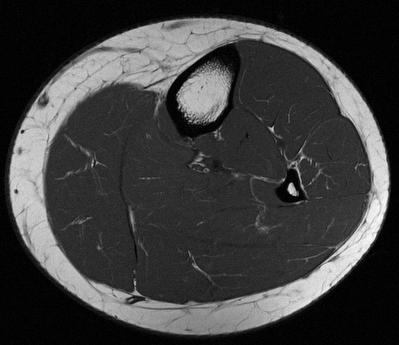
\includegraphics[height=3.25cm]{jambe}
\caption{Leg.}
\label{fig:image_restoration_denoising:enonce:leg}
\end{figure}

\section{Generation of random noises}
\index{Noise!Uniform}
\index{Noise!Gaussian}
\index{Noise!Salt \& Pepper}
\index{Noise!Exponential}

Some random noises are defined with the given functions (corresponding to specific distributions): 
\begin{itemize}
	\item uniform noise: $R=a+(b-a)*U(0,1)$. 
	\item Gaussian noise: $R=a+b*N(0,1)$.
	\item Salt and pepper noise: $R : \left\{\begin{array}{ccc}
	0\leq U(0,1)\leq a &\mapsto & 0\\
	a<U(0,1)\leq b&\mapsto & 0.5\\
	b< U(0,1)\leq 1 &\mapsto & 1
	\end{array}\right.$
	\item Exponential noise : $R=\displaystyle -\frac{1}{a}*\ln(1-U(0,1))$
\end{itemize}

\begin{qbox}
Generate sample images with the four kinds of random noise and visualize their histograms with the built-in functions. Pay attention to the intensity range of the resulting images when calculating the histograms
\end{qbox}

\begin{mcomment}
\begin{mremark}
The \matlabregistered{} functions \minline{rand} and \minline{randn} are used to generate random numbers with uniform and normal laws, respectively. The \minline{imhist}
function displays the image histogram. The \minline{imadjust} functions can be useful in order to adjust the values of the image and get a correct display.
\end{mremark}
\end{mcomment}


\section{Noise estimation}
The objective is to evaluate the characteristics of the noise in a damaged/noisy image (in a synthetic manner in this tutorial).
\begin{qbox}
\begin{enumerate}
	\item Visualize the histogram of a Region Of Interest (ROI) of the image of Fig.\ref{fig:image_restoration_denoising:enonce:leg}.
	The ROI should be extracted from a uniform (intensity) region. 
	\item Add an exponential noise to the original image and visualize the histogram of the selected ROI.
	\item Add a Gaussian noise to the original image and visualize the histogram of the selected ROI.
\end{enumerate}
\end{qbox}
\begin{mcomment}
\begin{mremark}
The  function \minline{imnoise} adds a specific noise on an image. The function \minline{roipoly} specifies a polygonal Region of Interest.
\end{mremark}
\end{mcomment}


\section{Image restoration by spatial filtering}
\index{Restoration!Median filter}
\begin{qbox}
\begin{enumerate}
	\item Add a salt-and-pepper noise to the image of Fig.\ref{fig:image_restoration_denoising:enonce:leg}. 
	\item Test the 'min', 'max', 'mean' and 'median' image filters. 
	\end{enumerate}	
\end{qbox}
\begin{mcomment}
\begin{mremark}
 Use the  function \minline{imnoise} to add noise to an image. See \minline{imfilter}, \minline{ordfilt2} and \minline{medfilt2}.
\end{mremark}
\end{mcomment}

\begin{pcomment}
\begin{premark}
See the module \pinline{scipy.ndimage}
\end{premark}
\end{pcomment}



The median filter is efficient in the case of salt-and-pepper noise. However, it replaces every pixel value (first problem) by the median value determined at a given scale (second problem). In order to avoid these two problems, Gonzalez and Woods proposed an algorithm \cite{Gonzalez2002}. 
\index{Restoration!Adaptive median filter}

\begin{algorithm}[H]
\KwData{Input (noisy) image $I$}
\KwData{Maximal scale $S_{max}$}
\KwResult{Filtered image $F$}
\SetKwData{Smax}{$S_{max}$} 
\SetKwFunction{amf}{amf}
\SetKwProg{Fn}{Function}{:}{}
\SetKwProg{FMain}{Main Function}{:}{}
\SetKwFunction{FindScale}{FindScale}
\SetKwFunction{MedFilter}{Med}
\SetKwFunction{OR}{OR}
\SetKwFunction{MinFilter}{Min}
\SetKwFunction{MaxFilter}{Max}
\SetKwFunction{isMedImpulseNoise}{isMedImpulseNoise}
\DontPrintSemicolon
\;
\FMain{\amf{$I$, $S_{max}$}}{
\ForAll{pixels $(i,j)$}{
	
$S\leftarrow 1$\;
\While{\isMedImpulseNoise{$I$, $i$, $j$, $S$} AND $S\leq S_{max}$}
{
	$S\leftarrow S+1$\;
	$med\leftarrow \MedFilter(I, i, j, S)$\;
}
	\eIf{$I(i,j)=$\MinFilter{$I$, $i$, $j$, $S$} \OR $I(i,j)=$\MaxFilter{$I$, $i$, $j$, $S$} \OR $S=S_{max}$}{$F(i,j)\leftarrow$ \MedFilter{$I$, $i$, $j$, $S$}\;}
	{$F(i,j)\leftarrow I(i,j)$}
}
}
\caption{Adaptive median filter \cite{Gonzalez2002}. The main function takes two arguments: the image $I$ to be filtered and the maximal size of neighborhood $S_{max}$. For each pixel $(i,j)$, the good scale is the scale where the median value is different from the min and the max (median value is thus not an impulse noise). Then, if the pixel value is an impulse noise or the maximal scale has been reached, it must be filtered. Otherwise, it is kept untouched. Min, Max and Med functions compute the minimum, maximum and the median value in a neighborhood of size $S$ centered at a pixel $(i,j)$ in image $I$.}
\label{algo:denoising:enonce:amf}
\end{algorithm}

\setcounter{algocf}{0}
\begin{algorithm}
\SetKwFunction{isMedImpulseNoise}{isMedImpulseNoise}
\SetKwProg{Fn}{Function}{:}{}
\DontPrintSemicolon
\Fn{\isMedImpulseNoise{$I$, $i$, $j$, $S$}}{
		$med\leftarrow \MedFilter(I, i, j, S)$\;
		\eIf{med=\MaxFilter{$I$, $i$, $j$, $S$} \OR med=\MinFilter{$I$, $i$, $j$, $S$}}{
			\KwRet True\;
		}{\KwRet False\;}
	}
\caption{End.}
\end{algorithm}


\begin{qbox}Implement the adaptive median filter from the following algorithm (Alg.\ref{algo:denoising:enonce:amf}) based on two steps (the operator acts on an operational window of size $k\times k$ where different statistics are calculated: median, min or max).

\end{qbox}

